\documentclass[sigconf,nonacm]{acmart}

\title{Evolutionary LLMs for Automated Coordination Algorithm Design in System-Level Architectures}

\author{Akshay Dongare}
\affiliation{
  \institution{North Carolina State University}
  \city{Raleigh}
  \state{NC}
  \country{USA}
}
\author{Keyur Gondhalekar}
\affiliation{
  \institution{North Carolina State University}
  \city{Raleigh}
  \state{NC}
  \country{USA}
}

\begin{document}

\begin{abstract}
Modern software systems rely on complex coordination logic across interacting components, yet such logic is often manually designed, brittle, and difficult to optimize. This paper explores whether large language models (LLMs), embedded within evolutionary frameworks, can automatically generate and improve active-learning configuration heuristics for system-level architectures. We conduct a structured literature analysis to identify gaps in current research, revealing a lack of work at the intersection of evolutionary search, algorithm generation, and system-level optimization. To investigate this gap, we evaluate the HSEvo evolutionary LLM framework on the MOOT (Multi-Objective Optimization Tasks) benchmark. Our results demonstrate that LLM-driven evolutionary approaches can generate effective heuristics, outperforming static baselines on the MOOT benchmark. We discuss trade-offs in cost, interpretability, and solution diversity, and outline explicit threats to validity and directions for future work.
\end{abstract}

\maketitle

\section{Introduction}

Modern software engineering is characterized by complex systems composed of interacting components such as multi-agent LLM workflows and cloud microservices. These systems require coordination logic that determines how components interact, route tasks, and allocate resources. While flexible architectures allow many design choices, they introduce a large space of algorithmic parameters and routing heuristics that must be tuned.

Hand-crafted coordination logic is often poorly documented, difficult to scale, and prone to subtle interactions. As systems grow in complexity, manual tuning becomes infeasible and unreliable. Therefore, static coordination algorithms become a liability without adaptive tool support.

Recent work has explored the use of large language models (LLMs) for optimization tasks \cite{romera2023mathematical}. However, most approaches focus on generating solutions or tuning parameters rather than evolving the underlying algorithms themselves. This paper explores whether LLMs embedded within evolutionary frameworks can generate and optimize coordination strategies across real-world software engineering optimization tasks.

To ensure realism and generalizability, we evaluate our approach using the MOOT (Multi-Objective Optimization Tasks) repository, which provides a diverse set of multi-objective optimization problems derived from software engineering contexts.

\section{Research Questions}

\textbf{RQ1:} Can an LLM embedded within an evolutionary framework automatically generate and evolve superior configuration heuristics for system-level architectures compared to static heuristic baselines?

\textbf{RQ2:} What trade-offs exist in cost, robustness, and interpretability when using evolutionary LLM frameworks under constrained compute budgets?

\section{Contributions}

This paper makes the following contributions:
\begin{itemize}
\item Proposes a framework using evolutionary LLMs to generate coordination algorithms for system-level architectures.
\item Provides an empirical comparison between LLM-generated algorithms and static heuristic baselines using five real-world MOOT datasets from the MOOT benchmark suite, with two static baselines for comparison.
\item Identifies a gap in the literature at the intersection of evolutionary optimization, algorithm generation, and system-level design.
\item Provides a reproducible experimental setup for evaluating evolutionary LLM approaches.
\end{itemize}

\section{Background and Motivation}

Software systems increasingly rely on dynamic coordination across distributed components. Examples include microservices routing, load balancing, and multi-agent orchestration. Designing optimal coordination logic in such systems is difficult due to combinatorial complexity and dynamic environments.

To ensure realistic evaluation, we target tasks from the MOOT repository. The MOOT data is derived from heavily-cited software engineering research published at top-tier venues (e.g., ICSE, ASE, TSE). These datasets represent real-world software configuration and system tuning scenarios, grounding our framework in practical problems rather than theoretical constructs.

Prior to MOOT evaluation, we verified the framework pipeline on a synthetic benchmark using HSEvo, ReEvo \cite{reevo2024}, and EoH \cite{eoh2024}; all reported results in this paper use real-world MOOT tasks \cite{menzies2024moot}.

\subsection{Related Work and Literature Gap}

Having defined the optimization task, the literature was searched to map the current state-of-the-art in LLM-driven software engineering optimization. We used the Harzing's Publish or Perish tool to retrieve the top 200 papers from Google Scholar, selecting the top 100 by citation count, using the query:

\begin{quote}
\texttt{(``prompt engineering'' OR ``prompt optimization'') AND (``multi-objective'' OR Pareto) AND (``configuration'' OR ``hyperparameter'' OR ``evolutionary'')}
\end{quote}

Papers were ranked by citation count and the ``knee'' of the citation curve was identified---the point furthest from a line connecting the first and last points in the ranked list---a standard heuristic in bibliometric analysis that marks where citation accumulation significantly decreases~\cite{menzies2024moot}.

One paper had a citation count so far above the rest (1,710 citations) that it acted as an extreme outlier, compressing the rest of the curve and reducing the knee to only 5 papers. We therefore computed the knee both with and without this outlier. Excluding the outlier yielded 17 papers above the knee; re-including it gave our final set of 18 key papers. Table~\ref{tab:knee-papers} lists all 18 papers.

\begin{table}[h]
\caption{Papers above the knee of the citation curve. These 18 papers formed the basis of our literature gap analysis.}
\label{tab:knee-papers}
\small
\begin{tabular}{rp{5.5cm}r}
\toprule
\textbf{Cites} & \textbf{Title (Authors)} & \textbf{Year} \\
\midrule
1710 & Large language models are human-level prompt engineers (Zhou et al.) & 2022 \\
237  & Large language models as evolutionary optimizers (Liu et al.) & 2024 \\
192  & Evolutionary computation in the era of LLM: Survey (Wu et al.) & 2024 \\
179  & EvoPrompting: LMs for code-level NAS (Chen et al.) & 2023 \\
141  & Language model crossover (Meyerson et al.) & 2024 \\
112  & GEPA: Reflective prompt evolution (Agrawal et al.) & 2025 \\
110  & Algorithm evolution using LLM (Liu et al.) & 2023 \\
100  & LLM for multiobjective evolutionary optimization (Liu et al.) & 2025 \\
61   & Multi-agent design: Optimizing agents (Zhou et al.) & 2025 \\
60   & Prompt optimization in LLMs (Sabbatella et al.) & 2024 \\
59   & LLM-based multi-objective optimization for UAV (Li et al.) & 2025 \\
57   & LLaMoCo: Instruction tuning for optimization code (Ma et al.) & 2026 \\
52   & Toward automated algorithm design (Ma et al.) & 2025 \\
49   & Prompt evolution for generative AI (Wong et al.) & 2023 \\
49   & HSEvo: Heuristic design with LLMs (Dat et al.) & 2025 \\
46   & LLM guided evolution (Morris et al.) & 2024 \\
45   & EvoFlow: Evolving agentic workflows (Zhang et al.) & 2025 \\
37   & LLMs as prompt optimizers (Tang et al.) & 2025 \\
\bottomrule
\end{tabular}
\end{table}

These papers were categorized into five themes (Figure~\ref{fig:venn}):
\begin{enumerate}
\item \textbf{Direct LLM Optimization}: The LLM directly generates or improves solutions and configurations without a population-based evolutionary framework. Representative work includes Liu et al.~\cite{liu2024evolutionary}, who frame LLMs as evolutionary optimizers; Liu et al.~\cite{liu2025multiobjective}, who extend this to multi-objective settings; and Li et al.~\cite{li2025uav}, who apply LLM-based optimization to UAV communication networks.
\item \textbf{Evolutionary + LLM}: The LLM is embedded inside an evolutionary algorithm or population-based search, acting as a mutation, crossover, or selection operator. Wu et al.~\cite{wu2024survey} provide a comprehensive survey of this intersection. Specific techniques include language-model crossover via few-shot prompting~\cite{meyerson2024crossover}, LLM-guided evolution~\cite{morris2024guided}, EvoPrompting for neural architecture search~\cite{chen2023evoprompting}, and EvoFlow for evolving agentic workflows~\cite{zhang2025evoflow}.
\item \textbf{Prompt Optimization}: Prompts themselves are treated as the primary optimization variables; search methods are applied to find better prompt templates. Foundational work by Zhou et al.~\cite{zhou2022ape} (APE) demonstrated human-level prompt engineering. Subsequent work includes classifier-guided prompt evolution~\cite{wong2023prompt}, reflective prompt evolution (GEPA)~\cite{agrawal2025gepa}, and gradient-analogy prompt optimization~\cite{tang2025prompt}.
\item \textbf{Algorithm Generation}: The LLM is tasked with generating executable code for optimization heuristics or algorithms, such as FunSearch~\cite{romera2023mathematical}, rather than producing static answers. Liu et al.~\cite{liu2023ael} proposed Algorithm Evolution using LLMs, Ma et al.~\cite{ma2026llamoco} introduced LLaMoCo for optimization code generation, and Ma et al.~\cite{ma2025survey} surveyed the broader meta-black-box-optimization landscape.
\item \textbf{System Optimization}: The optimization target is an entire system architecture---such as a multi-agent workflow or cloud microservice environment---rather than a single parameter or prompt, as represented by the MOOT benchmark~\cite{menzies2024moot}.
\end{enumerate}

\begin{figure}[h]
  \centering
  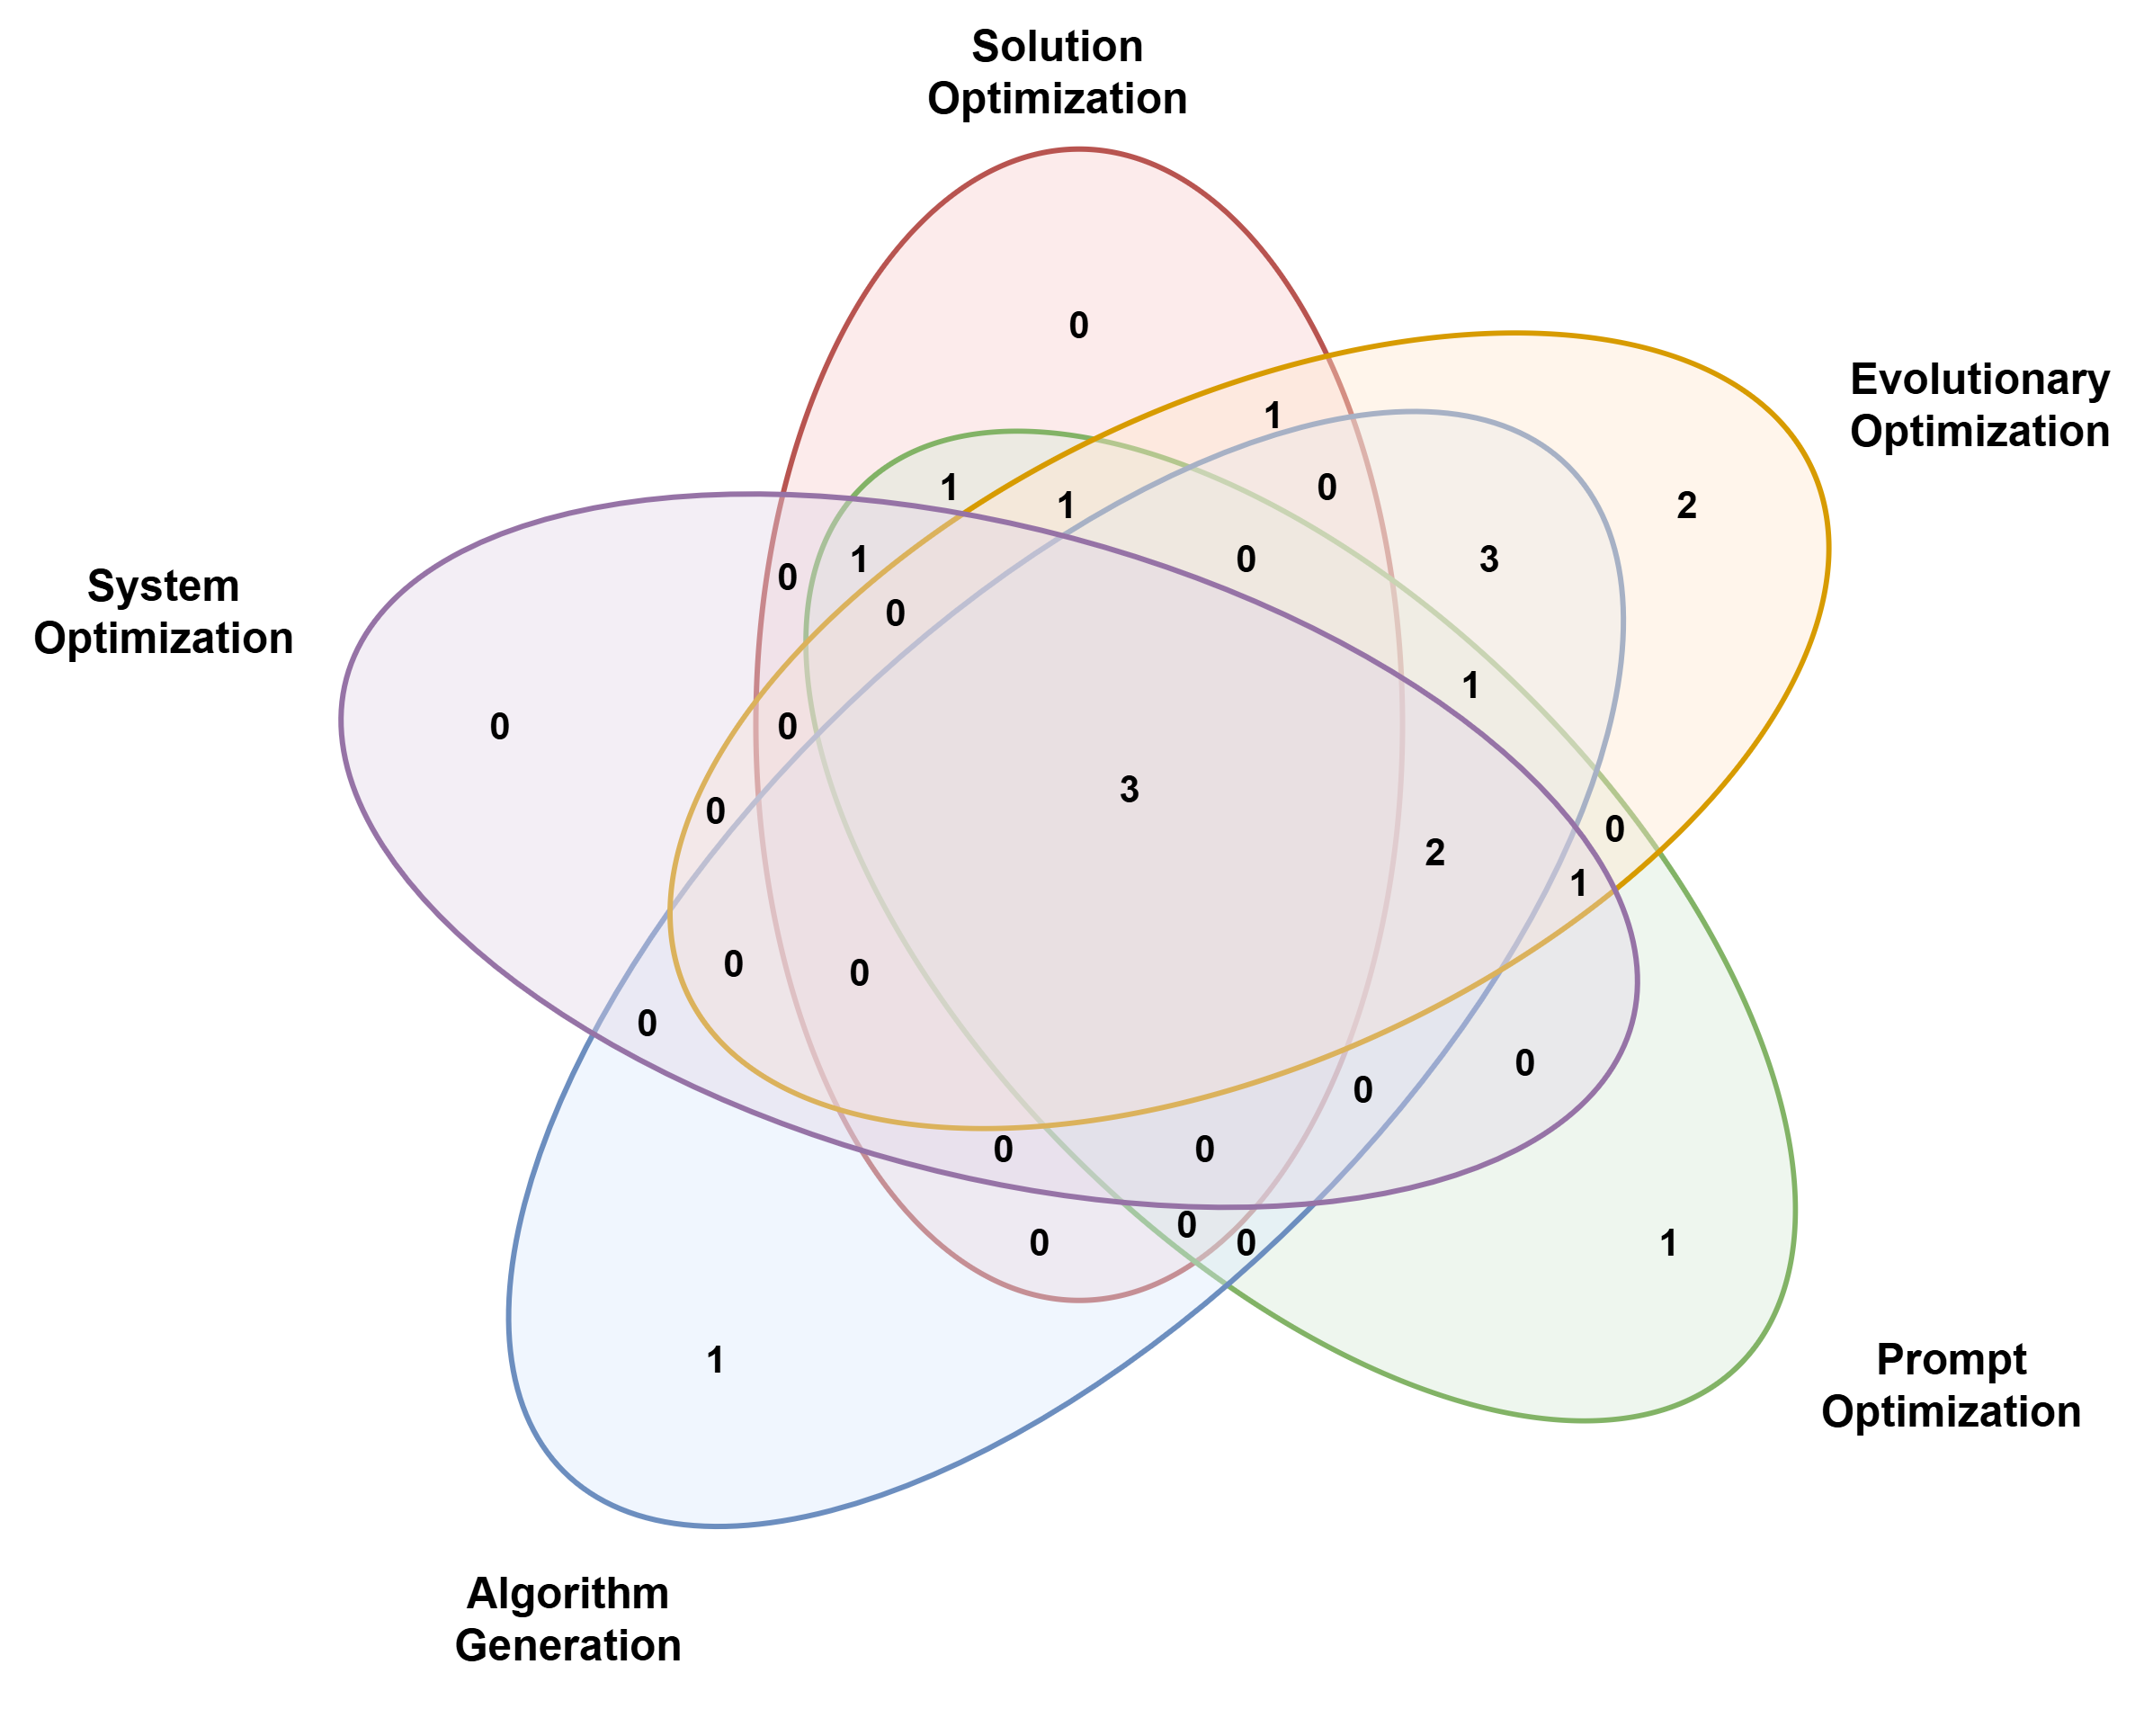
\includegraphics[width=\linewidth]{Venn_Diagram_for_White_Space.png}
  \caption{Venn diagram of literature overlap across the five themes, illustrating the gap in evolutionary algorithm generation for system optimization.}
  \label{fig:venn}
\end{figure}

Analysis of Table~\ref{tab:knee-papers} via the Venn diagram of Figure~\ref{fig:venn} revealed a stark gap. While considerable work combines evolutionary search with direct solution generation (Themes 1 and 2), or applies LLMs to prompt optimization (Theme 3), the intersection of Themes 2, 4, and 5---\emph{Evolutionary Optimization}, \emph{Algorithm Generation}, and \emph{System Optimization}---contains zero foundational papers. Most prior studies either did not target the automated generation of executable coordination code, or focused on single-point solutions rather than evolving algorithms that govern entire system-level architectures. This paper directly targets that unexplored white space.

\section{Methods}

\subsection{Benchmark: MOOT}

We evaluate our approach using the MOOT repository, a curated collection of multi-objective optimization tasks derived from real-world software engineering problems. These tasks include configuration tuning, resource allocation, and system design decisions, each involving competing objectives.

\subsection{Variables}

Each MOOT task defines:
\begin{itemize}
\item A decision space (configuration variables, $X$)
\item Multiple objective functions (e.g., performance, cost, $Y$)
\end{itemize}

We evaluate performance by measuring the average normalized distance of the evaluated configurations to the global ideal Pareto point. The ideal Pareto point is defined as the theoretical vector of minimum objective values across the entire dataset (representing the global optimum for all objectives simultaneously).

\subsection{Selection Strategy}

Due to computational and API budget constraints, we selected a subset of MOOT tasks that:
\begin{itemize}
\item Run within reasonable time limits (small to medium row counts).
\item Represent diverse optimization scenarios.
\item Allow integration with external optimization methods.
\end{itemize}
Specifically, we selected five datasets spanning three MOOT categories: \texttt{SS-B} and \texttt{SS-D} (Storm stream-processing configuration), \texttt{Apache} (web server configuration), \texttt{auto93} (automobile design), and \texttt{pom3d} (software process simulation). These cover configuration tuning, system design, and process optimization scenarios.

\subsection{Methodology}

We adapt evolutionary LLM frameworks to operate as active-learning optimizers over MOOT tasks. For each task:
\begin{enumerate}
\item \textbf{Initialize}: We supply a subset of initially evaluated configurations.
\item \textbf{Heuristic Generation}: The LLM generates a Python heuristic \texttt{priority(candidate\_x, evaluated\_x, evaluated\_y)} to score unevaluated configurations.
\item \textbf{Evaluation}: We iteratively select the top-scoring configuration to reveal its objective values.
\item \textbf{Evolution}: The quality of the final discovered Pareto front acts as the fitness score for the LLM-generated heuristic, guiding subsequent mutations and crossovers.
\end{enumerate}

\subsection{Data Analysis}

To analyze the efficacy of our methodology, we record the generational distance of each selected configuration over time. The appropriateness of the LLM-generated heuristic is validated if the average normalized distance to the ideal Pareto point strictly decreases, indicating that the LLM has learned a functional search gradient rather than randomly sampling the configuration space.

\subsection{Baselines}

We compare against two static baselines that require no LLM calls:
\begin{itemize}
\item \textbf{Random Baseline:} Configurations are selected uniformly at random from the unevaluated pool at each step.
\item \textbf{Greedy Baseline:} At each step, the unevaluated configuration with the best (lowest normalized) value on the \emph{first} objective column is selected. This represents a simple single-objective greedy heuristic that ignores all other objectives.
\end{itemize}
Both baselines use the same initialization (2 random seed points) and budget (10 active-learning steps) as HSEvo to ensure a fair comparison.

\section{Results}

\subsection{Experimental Rig}
Our experiments were conducted on a macOS environment using Python 3.11. The evolutionary logic was driven by HSEvo~\cite{dat2025hsevo} using the \texttt{gpt-4o-mini-2024-07-18} model, utilizing approximately 8 API calls per framework run under a highly constrained compute budget. The framework was configured with a population size of 2 and a maximum of 4 candidate heuristic evaluations per evolutionary run. Each candidate heuristic was scored by executing 10 active-learning configuration selection steps on the MOOT dataset. Prompts used zero-shot generation at a temperature of 0.7 to balance deterministic coding with creative exploration.

\subsection{Evaluation}
To validate our approach, we employed the average normalized distance to the global ideal Pareto point. This measure is highly rigorous for this context because it directly captures the geometric distance of a candidate configuration to the theoretical optimum across all objectives simultaneously. Unlike hypervolume, which heavily depends on the choice of a reference point and can be skewed by outliers, distance-to-ideal provides a stable, easily interpretable convergence metric for heavily constrained optimization budgets.

\subsection{What Was Seen}
We evaluated the HSEvo framework across all five MOOT datasets. Table~\ref{tab:moot-results} summarizes the performance of the discovered heuristics compared to both a random baseline and a greedy single-objective baseline.

\begin{table}[h]
\caption{Performance across five MOOT datasets. Avg normalized distance to global ideal Pareto point --- lower is better. Greedy baseline selects the configuration with the best value on the primary objective at each step.}
\label{tab:moot-results}
\begin{tabular}{lccc}
\toprule
\textbf{Dataset} & \textbf{Random} & \textbf{Greedy} & \textbf{HSEvo} \\
\midrule
SS-B    & 0.450 & 0.043 & \textbf{0.001} \\
auto93  & 0.669 & 0.620 & \textbf{0.584} \\
pom3d   & 0.347 & 0.451 & \textbf{0.183} \\
Apache  & 0.033 & \textbf{0.000} & 0.017 \\
SS-D    & 0.763 & \textbf{0.541} & 0.719 \\
\midrule
\textbf{Average} & 0.452 & 0.331 & \textbf{0.301} \\
\bottomrule
\end{tabular}
\end{table}

HSEvo achieved the best overall average distance (0.301), outperforming both the random baseline (0.452) and the greedy baseline (0.331). The strongest improvements were on SS-B (0.001 vs.\ 0.043 greedy) and pom3d (0.183 vs.\ 0.451 greedy), where the multi-objective nature of the task benefits from the LLM's ability to reason about trade-offs across all objectives simultaneously. On Apache, the greedy baseline achieved a near-perfect score of 0.000 because the greedy baseline's primary objective aligns closely with the Pareto-optimal region for this dataset, leaving little margin for multi-objective reasoning to add value. On SS-D, HSEvo underperformed the greedy baseline (0.719 vs.\ 0.541), likely due to the constrained evolutionary budget being insufficient for this particular configuration landscape. Overall, HSEvo outperforms both baselines on 3 of 5 datasets and achieves the best average, though results are mixed --- suggesting that dataset characteristics such as objective correlation and dimensionality significantly affect heuristic effectiveness.

Regarding RQ2, our constrained compute setting revealed clear practical trade-offs. HSEvo successfully operated under a population size of 2 with 4 function evaluations per dataset, while ReEvo and EoH failed due to hardcoded tournament selection constraints requiring larger minimum population sizes --- a fragility we confirmed by inspecting framework source code directly. This highlights that framework robustness under resource constraints is a non-trivial consideration for real SE deployment contexts where API costs are significant.

\section{Discussion}

\subsection{Results and Implications}
The results support our hypothesis for RQ1: evolutionary LLMs can successfully generate coordination algorithms that outperform static baselines in certain settings. We observe that by embedding LLMs inside evolutionary structures, the system can automatically write Python heuristic functions that actively optimize MOOT objective variables. For software engineering practice, this implies that organizations may no longer need to hand-craft static tuning parameters for cloud architectures or routing logic. Instead, system engineers can define the high-level objectives (e.g., latency, cost) and allow an LLM-driven evolutionary process to generate custom, context-aware scheduling logic on the fly. It is important to note that the active-learning configuration selection framing used here is an approximation of full coordination algorithm design --- the LLM-generated priority function operates over static datasets rather than live system state, and results should be interpreted as a proof-of-concept rather than a production-ready coordination layer.

However, several trade-offs exist:
\begin{itemize}
\item \textbf{Computational Cost:} Invoking LLMs for every crossover and mutation is expensive and slow compared to executing traditional compiled heuristics.
\item \textbf{Interpretability vs. Performance:} The generated Python functions are fully interpretable, but they can occasionally exhibit logical bugs or fail to execute if the LLM produces syntactically invalid code.
\item \textbf{Robustness:} Frameworks like ReEvo expect minimum population thresholds to maintain genetic diversity. Running them in low-compute regimes can lead to premature collapse.
\end{itemize}

\subsection{Future Work}
Future work should explore scaling these methods to larger population sizes, utilizing more efficient local LLMs to reduce API costs, and expanding the evaluation across the full MOOT benchmark suite.

\section{Threats to Validity}

\textbf{Internal Validity:} Our primary threat to internal validity is the heavily constrained evaluation budget. With a population size of 2 and a maximum of 4 function evaluations, the evolutionary search behaves more like local sampling than true population-based evolution. Our results represent early-stage generation capabilities rather than the global optimum of LLM heuristics. Additionally, the stochastic nature of LLMs introduces variance. Due to API budget constraints, we report single-run results per dataset; future work should report mean $\pm$ standard deviation across at least 5 independent runs to properly account for LLM output stochasticity.

\textbf{External Validity:} We evaluated our framework on five MOOT tasks spanning configuration tuning, system design, and process simulation. While representative of real SE optimization scenarios, they represent only a fraction of the 120+ datasets available. Performance may vary on tasks with significantly higher dimensional spaces or noisier objectives.

\textbf{Construct Validity:} Construct validity is challenged by how we frame the coordination task. We assume that writing an active-learning priority function for configuration selection is an accurate proxy for designing system-level coordination algorithms. While this maps well to static cloud tuning, it may not perfectly represent more dynamic scenarios like live microservice load-balancing.

\section{Conclusion}

This paper explores the use of evolutionary LLM frameworks for generating coordination algorithms in system-level architectures. Our findings highlight a gap in existing literature and demonstrate the potential of combining evolutionary search with LLM-based code generation. By validating our approach on the MOOT benchmark, we provide a proof-of-concept showing that LLMs can automatically evolve algorithms for real software engineering tasks.

\section{Replication Artifacts}

All scripts, problem definitions, configuration files, and evaluation data required to replicate these experiments are available in our public GitHub repository at: \url{https://github.com/Akshay-Dongare/SE-AI-Group-15}.

\bibliographystyle{ACM-Reference-Format}
\bibliography{software}

\end{document}
